\documentclass[a4paper,12pt]{article}
\usepackage[a4paper,top=1.3cm,bottom=2cm,left=1.5cm,right=1.5cm,marginparwidth=0.75cm]{geometry}
\usepackage{setspace}
\usepackage{cmap}
\usepackage{mathtext}
\usepackage[T2A]{fontenc}
\usepackage[utf8]{inputenc}
\usepackage[english,russian]{babel}
\usepackage{multirow}
\usepackage{graphicx}
\usepackage{wrapfig}
\usepackage{tabularx}
\usepackage{float}
\usepackage{longtable}
\usepackage{hyperref}
\hypersetup{colorlinks=true,urlcolor=blue}
\usepackage[rgb]{xcolor}
\usepackage{amsmath,amsfonts,amssymb,amsthm,mathtools}
\usepackage{icomma}
\mathtoolsset{showonlyrefs=true}
\usepackage{euscript}
\usepackage{mathrsfs}
\usepackage{float}
\setlength{\parindent}{1cm} % Устанавливает отступ в 1.5 см для всех абзацев


\DeclareMathOperator{\sgn}{\mathop{sgn}}
\newcommand*{\hm}[1]{#1\nobreak\discretionary{}
	{\hbox{$\mathsurround=0pt #1$}}{}}

\title{\textbf{Отчёт о выполненой лабораторной работе \\ \textit{Измерение теплопроводности
воздуха при постоянном давлении (2.2.3)}}}

\author{Каплин Артём Б01-402}
\date{1 марта 2025}

\begin{document}

\maketitle

	\section{Аннотация}

	\textbf{Цель работы:} измерить коэффициент теплопроводности воздуха при атмосферном
        давлении в зависимости от температуры. \\
\newline
	\textbf{Оборудование:}  цилиндрическая колба с натянутой по оси платиновой нитью; термостат;
        вольтметр и амперметр; источник
        постоянного напряжения; магазин сопротивлений.

	\section{Теоретические сведения}

        Теплопроводность — это процесс передачи тепловой энергии от нагретых
частей системы к холодным за счёт хаотического движения частиц среды . В газах теплопроводность осуществляется за счёт непосредственной передачи кинетической энергии от быстрых молекул к медленным при их столкновениях. Перенос тепла описывается законом Фурье, утверждающим, что плотность потока энергии $\vec{q}$ (количество теплоты, переносимое через единичную площадку в единицу времени) пропорциональна градиенту температуры $\nabla T$:
\[
\vec{q} = -\kappa \cdot \nabla T, \tag{1} \label{1}
\]
где $\kappa$ — \textit{коэффициент теплопроводности}.

МКТ даёт следующую оценку для коэффициента теплопроводности газов:
\[
\kappa \sim \lambda \vec{v} \cdot n c_V, \tag{2}
\]
где $\lambda$ — длина свободного пробега молекул газа, $ \vec{v} = \sqrt{\frac{8 k_{\text{Б}} T}{\pi m}}$ — средняя скорость их теплового движения, $n$ — концентрация (объёмная плотность) газа, $c_V = \frac{i}{2} k_{\text{Б}}$
— его теплоёмкость при постоянном объёме в расчёте на одну молекулу ($i$ — число степеней свободы молекулы).


Рассмотрим стационарную теплопроводность в цилиндрической геометрии. Пусть тонкая нить радиусом $r_1$ и длиной $L$ помещена на оси цилиндра радиусом $r_0$. Температура стенок цилиндра $T_0$ поддерживается постоянной. Пусть в нити выделяется некоторая тепловая мощность $Q$ [Вт]. Если цилиндр длинный ($L \gg r_0$), можно пренебречь теплоотводом через его торцы. Тогда все параметры газа можно считать зависящими только от расстояния до оси системы $r$, а поток тепла $\vec{q}$ направлен строго радиально. Вместо первой формулы имеем скалярное уравнение
\[
q = -\kappa \frac{dT}{dr}. \tag{3}
\]
В стационарном состоянии полный поток тепла через любую цилиндрическую поверхность радиуса $r$ площадью $S = 2 \pi r L$ должен быть одинаков и равен $Q$:
\[
Q = -2 \pi L \cdot \kappa \frac{dT}{dr} = \text{const}. \tag{4}
\]
Если перепад температуры $\Delta T = T_1 - T_0$ между нитью и стенками цилиндра мал ($\Delta T \ll T_0$), то в (4) можно пренебречь изменением теплопроводности от температуры в пределах системы, положив $\kappa \approx \kappa(T_0)$. Тогда, разделяя переменные  и интегрируя от радиуса нити до радиуса колбы, получим
\[
Q = 2 \pi L \frac{\kappa \Delta T}{\ln(r_0/r_1)}. \tag{5}
\]


        \subsection{Эксперименатльная установка} 
        
        \begin{wrapfigure}{r}{0.4\textwidth}
        \begin{center}
            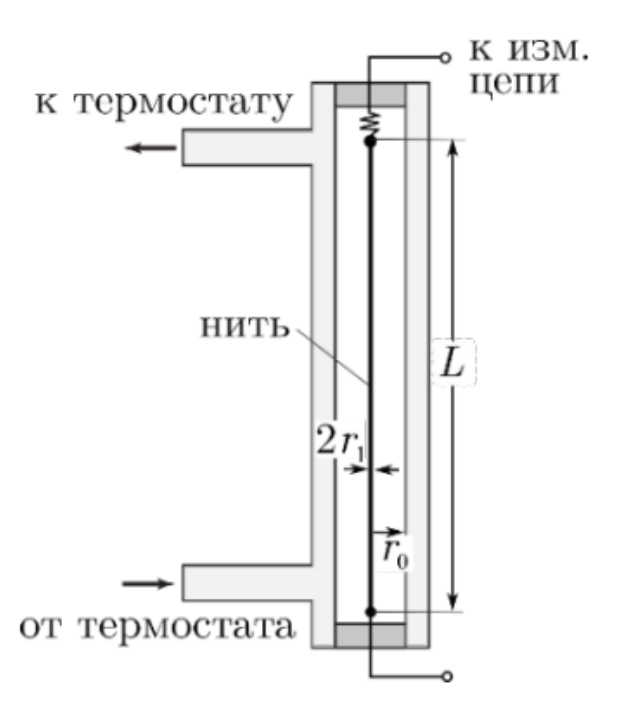
\includegraphics[width = 0.3\textwidth]{ustanovka.png}
        \end{center}
        \textbf{\caption{Схема установки}}
        \end{wrapfigure}
        
        Схема установки приведена на рис. 1. На оси трубки с внутренним диаметром $2r_0 \sim 0,7$ см размещена платиновая нить диаметром $2r_1 \sim 0,05$ мм и длиной $L \sim 40$ см. Полость трубки заполнена воздухом (полость через небольшое отверстие сообщается с атмосферой). Стенки трубки помещены в кожух, через которых пропускается вода из термостата, так что их температура $t_0$ поддерживается постоянной. Для предотвращения конвекции трубка расположена вертикально. Платиновая нить служит как источником тепла, так и датчиком температуры (термометром сопротивления). По пропускаемому через нить постоянному току $I$ и напряжению $U$ на ней вычисляется мощность нагрева по закону Джоуля–Ленца: $Q = UI$, и сопротивление нити по закону Ома: $R = \dfrac{U}{I}$. Сопротивление нити является однозначной функцией её температуры $R (t)$.\\


        В схеме рис. 2 для измерения напряжения и тока используется два мультиметра, работающие в режимах вольтметра и амперметра соответственно.
        Подключение к нити $R_{\text{н}}$ осуществляется по четырёхпроводной схеме. По двум
        проводам (токовая пара $I_{\text{+}}$ и $I_{\text{-}}$) через сопротивление пропускается измерительный ток, а два других (потенциальная пара ($U_{\text{+}}$ и $U_{\text{-}}$) используются для
        параллельного подключения вольтметра. Заметим, что
        при такой схеме внутреннее сопротивление приборов и сопротивление подводящих проводов практически не влияет на измерения: сопротивление амперметра не влияет на результат вовсе, а сопротивление вольтметра составляет
        обычно $1-100 \ \text{МОм}$, что при $R_{\text{н}} \sim 10$ Ом вносит относительную ошибку не более $10^{-5}$.

        \begin{wrapfigure}{r}{0.4\textwidth}
        \begin{center}
            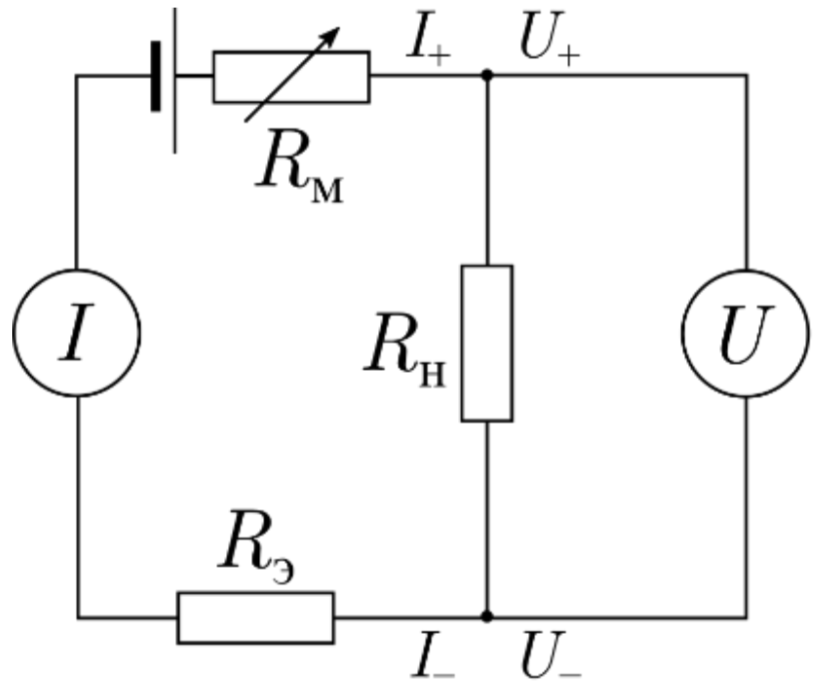
\includegraphics[width = 0.4\textwidth]{chain.png}
        \end{center}
        \caption{Электрическая схема измерения сопротивления нити и мощности нагрева}
        \end{wrapfigure}
        \newpage
        \subsection{Методика измерений}
        Принципиально неустранимая систематическая ошибка измерения температуры с помощью термометра сопротивления возникает из-за необходимости пропускать через резистор (нить) измерительный ток. Чем этот ток выше, тем с большей точностью будет измерен как он сам, так и напряжение. Однако при этом квадратично возрастает выделяющаяся на  резисторе мощность $Q = UI$. Следовательно, температура резистора становится выше, чем у объекта, температуру которого надо измерить. Измерения же при малых токах не дают достаточной точности. Эта проблема решается построением нагрузочной кривой - зависимости измеряемого сопротивления $R$ от выделяющейся в нём мощности $R(Q)$, с последующей экстраполяцией к нулевой мощности $Q \to 0$ для определения сопротивления $R_0 = R(0)$, при котором его температура равна температуре измеряемого объекта. Кроме того, в данной работе измерение нагрузочных кривых позволяет в ходе эксперимента получить температурную зависимость сопротивления нити, так как при $Q \to 0$ температура нити равна температуре термостата ($T \approx T_0$). В исследуемом интервале  (20-80 $^0C$) зависимость сопротивления от температуры можно с хорошей точностью аппроксимировать линейной функцией:

        \begin{align}
            R(t) = R_{273} \cdot (1 + \alpha t) \label{RT},
        \end{align}

        где $\alpha = \dfrac{1}{R_{273}} \dfrac{dR}{dT}$ - \textit{температурный коэффициент сопротивления материала}.


    \section{Приборы и данные}
    \begin{itemize}
    \item Магазин сопротивлений МЕГЕОН05350, погрешность  5\% 2\% 1\% 0,5\% \ для декад x0,1; x1; x10; x100 соответственно
    \item Мультиметры  АКИП В7-78/3, погрешность в режиме амперметра (0,15 \% ;\ 0,02 \text{мА}), в режиме вольтметра (0,004 \% ;\ 0,007 мВ)
    \item Источник питания
    \item Термостат жидкостный WCR-P12 (Daihan), погрешность 0,1 К
    \item Источник питания постоянного напряжения GW Instek GPS-2303 (0,5 \% \ ; 10 \text{мВ})
    \end{itemize}

    \section{Ход работы}
    \subsection{Предварителные расчёты}
    Оценим максимальную мощность нагрева $Q_{max} \ \text{[мВт]}$ , которую следует подавать на нить. Для оценки коэффициент теплопроводности воздуха примите равным $k \sim 25 \ \frac{\text{м} \cdot \text{Вт}}{\text{(м} \cdot \text{К)}}$. 
    Проведём предварительные расчёты параметров опыта. Сопротивление нити $R_{\text{н}} = 20 \ \text{Ом}$. 
    
     Получаем такую оценку: $Q_{max} \approx 381,4\ \text{мВт}$. Так же оцениваем максимальные ток и напряжение $I_{max} \approx 138,1 \ \text{мА}$; $U_{max} \approx 2,76 \ \text{В}$. В ходе работы не будем их превышать.

    \subsection{Подготовка экспериментальной устаноки}
        \begin{enumerate}
        \item  Проверяем, что измерительная цепь соответствует схеме.

        \item На магазине сопротивлений устанавливаем максимальное сопротивление, чтобы ток в цепи при её замыкании был минимален.

        \item По техническому описанию к установке включаем вольтметр и амперметр.

        \item Включаем источник питания. Убеждаемся, что напряжение на нём не превышает максимальное ($3 \ \text{В}$).

        \item Включаем термостат. Убеждаемся, что он находится при комнатной температуре ($23 \ ^oC$).
        \end{enumerate}

        \subsection{Проводим измерения}

         При комнатной температуре термостата измеряем зависимость сопротивления нити $R =\dfrac{U}{I}$ от подаваемой на неё мощности $Q = UI$. Понижая сопротивление на магазине, будем ждать около 30с для установления теплового равновесия. По окончании первой серии повысим температуру термостата. Для установления теплового равновесия будем ждать 5-7 минут. Сделаем 3 таких серии опытов. Результаты измерений представлены в таблицах. \\
         \newline

         \begin{table}[!ht]
    \begin{minipage}{0.48\linewidth}
        \centering
        \begin{tabular}{|c|c|c|c|}
            \hline
            $U, \, \text{мВ}$ & $I, \, \text{мА}$ & $R_н, \, \text{Ом}$ & $Q, \, \text{мВт}$\\ \hline
            $310$ & $15,73$ & $19,71$ & $4,9$ \\ \hline
            $560$ & $28,28$ & $19,80$ & $15,8$ \\ \hline
            $937$ & $47,00$ & $19,94$ & $44,0$ \\ \hline
            $1285$ & $63,76$ & $20,15$ & $81,9$ \\ \hline
            $2035$ & $97,88$ & $20,79$ & $199,2$ \\ \hline
            $2376$ & $112,28$ & $21,16$ & $266,8$ \\ \hline
           
        \end{tabular}
        \caption{Т термостата $23^\circ C$}
        \label{table_61}
    \end{minipage}
    \hspace{0.04\linewidth} % Параметр для отступа между таблицами
    \begin{minipage}{0.4\linewidth}
        \centering
        \begin{tabular}{|c|c|c|c|}
            \hline
            $U, \, \text{мВ}$ & $I, \, \text{мА}$ & $R_н, \, \text{Ом}$ & $Q, \, \text{мВт}$\\ \hline
            $354$ & $15,89$ & $22,28$ & $5,6$ \\ \hline
            $645$ & $28,84$ & $22,36$ & $18,6$ \\ \hline
            $960$ & $42,73$ & $22,47$ & $41,0$ \\ \hline
            $1271$ & $56,21$ & $22,61$ & $71,4$ \\ \hline
            $1879$ & $81,63$ & $23,02$ & $153,4$ \\ \hline
            $2458$ & $104,49$ & $23,52$ & $256,8$ \\ \hline
        \end{tabular}
        \caption{Т термостата $59 ^\circ C$}
        \label{table_80}
    \end{minipage}
\end{table}

         \begin{table}[!ht]
    \begin{minipage}{0.48\linewidth}
        \centering
        \begin{tabular}{|c|c|c|c|}
            \hline
            $U, \, \text{мВ}$ & $I, \, \text{мА}$ & $R_н, \, \text{Ом}$ & $Q, \, \text{мВт}$\\ \hline
            $ 324$ &  $16,04 $  &    $20,20$  &  $  5,2$ \\ \hline
            $ 595$ &  $29,32 $  &    $20,29$  &  $ 17,4$ \\ \hline
            $ 894$ &  $43,81 $  &    $20,41$  &  $ 39,2$ \\ \hline
            $1195$ &  $ 58,09$  &    $20,57$  &  $ 69,4$ \\ \hline
            $1799$ &  $ 85,53$  &    $21,03$  &  $153,9$ \\ \hline
            $2392$ &  $110,69$  &    $21,61$  &  $264,8$ \\ \hline
            $2649$ &  $120,96$  &    $21,90$  &  $320,4$ \\ \hline
            $2960$ &  $132,86$  &    $22,28$  &  $393,3$ \\ \hline
        \end{tabular}
        \caption{Т термостата $30 ^\circ C$}
        \label{table_61}
    \end{minipage}
    \hspace{0.04\linewidth} % Параметр для отступа между таблицами
    \begin{minipage}{0.4\linewidth}
        \centering
        \begin{tabular}{|c|c|c|c|}
            \hline
            $U, \, \text{мВ}$ & $I, \, \text{мА}$ & $R_н, \, \text{Ом}$ & $Q, \, \text{мВт}$\\ \hline
            $ 337$ &  $15,98 $   &      $21,09$  &  $  5,4$ \\ \hline
            $ 616$ &  $29,13 $   &      $21,15$  &  $ 17,9$ \\ \hline
            $ 922$ &  $43,36 $   &      $21,26$  &  $ 40,0$ \\ \hline
            $1228$ &  $ 57,29$   &      $21,43$  &  $ 70,4$ \\ \hline
            $1833$ &  $ 83,84$   &      $21,86$  &  $153,7$ \\ \hline
            $2421$ &  $108,02$   &      $22,41$  &  $261,5$ \\ \hline
            $2673$ &  $117,84$   &      $22,68$  &  $315,0$ \\ \hline
            $2977$ &  $129,26$   &      $23,03$  &  $384,8$ \\ \hline
        \end{tabular}
        \caption{Т термостата $42 ^\circ C$}
        \label{table_80}
    \end{minipage}
\end{table}
    \newpage
    \subsection{График зависимости сопротивления нити от мощности}
    Построим по МНК график зависимости $R(Q)$ и определим по нему $\frac{dR}{dQ}$ и $R_0$.


            \begin{table}[!ht]
                \centering
                \begin{tabular}{|c|c|c|}
                    \hline

                    $t, ^oC$ & $dR/dQ, \ \frac{\text{Ом}}{\text{Вт}}$ & $R_0, \ \text{Ом}$\\ \hline
                    $23$ & $(5,48 \pm 0,04)$ & $(19,6988 \pm 0,0046)$\\ \hline
                    $30$ & $(5,33 \pm 0,02)$ & $(20,1952 \pm 0,0050)$\\ \hline
                    $42$ & $(5,13 \pm 0,05)$ & $(21,0627 \pm 0,0038)$\\ \hline
                    $59$ & $(4,90 \pm 0,04)$ & $(22,2628 \pm 0,0031)$\\ \hline

                \end{tabular}
                \caption{Результаты: $dR/dQ$ и $R_0$ }
                \label{RQ_coeffs}
            \end{table}

    \begin{figure}[!ht]
        \begin{center}
            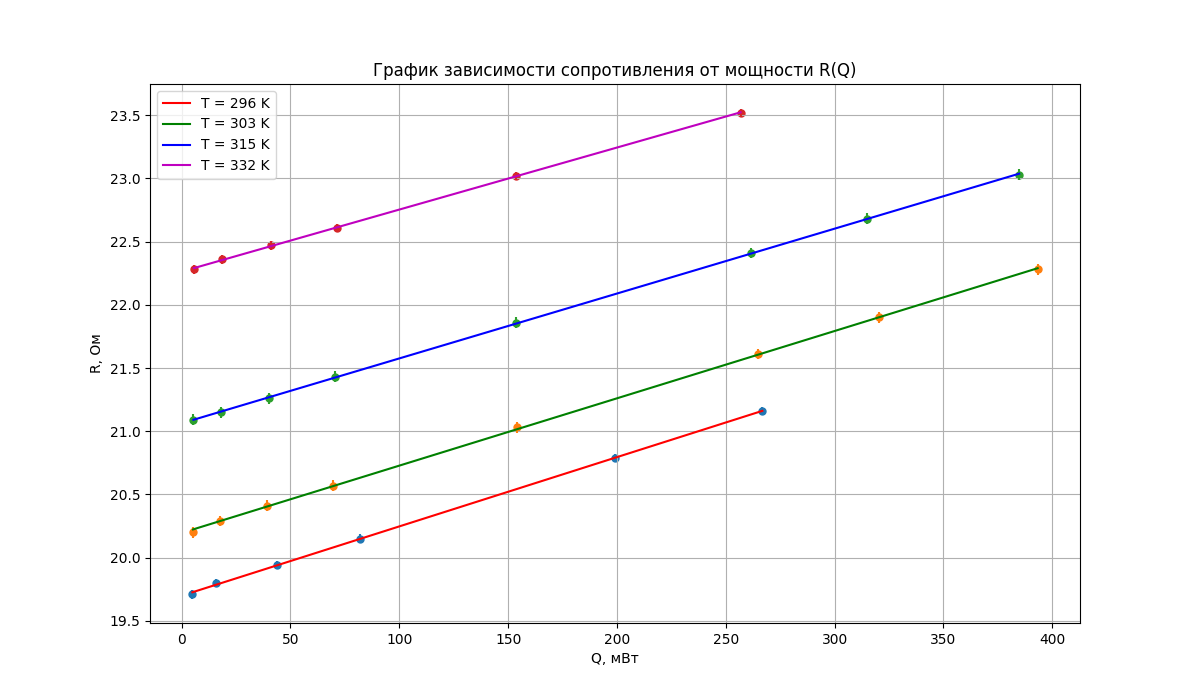
\includegraphics[width=1.1 \textwidth]{R(Q).png}
        \end{center}
    \end{figure}


        \subsection{График зависимости сопротивления нити от температуры}

            Также по МНК построим график зависимости $R_0(T)$, найдём $\frac{dR_0}{dT}$. Потом по формуле вычислим температурный коэфициент сопротивления $\alpha = \frac{1}{R_{273}}\cdot \frac{dR_0}{dT}$

           \[\frac{dR_0}{dT} = 71,30 \ \cdot 10^{-3} \ \frac{1}{\text{K}} \ \ \ \ \ \ \sigma_{\frac{dR_0}{dT}} = 0,18 \cdot 10^{-3} \ \frac{1}{\text{K}}  \ \ \ \ \ \   R_{273} = (18,06 \pm 0,06) \ \text{Ом}\]

          \[\alpha = (3,948 \pm 0,016)  \cdot 10^{-3} \ \frac{1}{\text{K}} \ \ \ \  \sigma_{\alpha} = \alpha \cdot \sqrt{\left( \frac{\sigma_{\frac{dR_0}{dT}}}{ \frac{dR_0}{dT}} \right)^2 + \left( \frac{\sigma_{R_{273}}}{R_{273}} \right)^2}\]

        \newline
        Результаты измерений оказались достаточно точными, мы видим, что температурный коэфициент сопротивления почти полностью совпадает с табличным значением для платины $Pt$, равным $3,9  \cdot 10^{-3} \ \frac{1}{\text{K}}$
        \newpage
            \begin{figure}[ht]
                \center{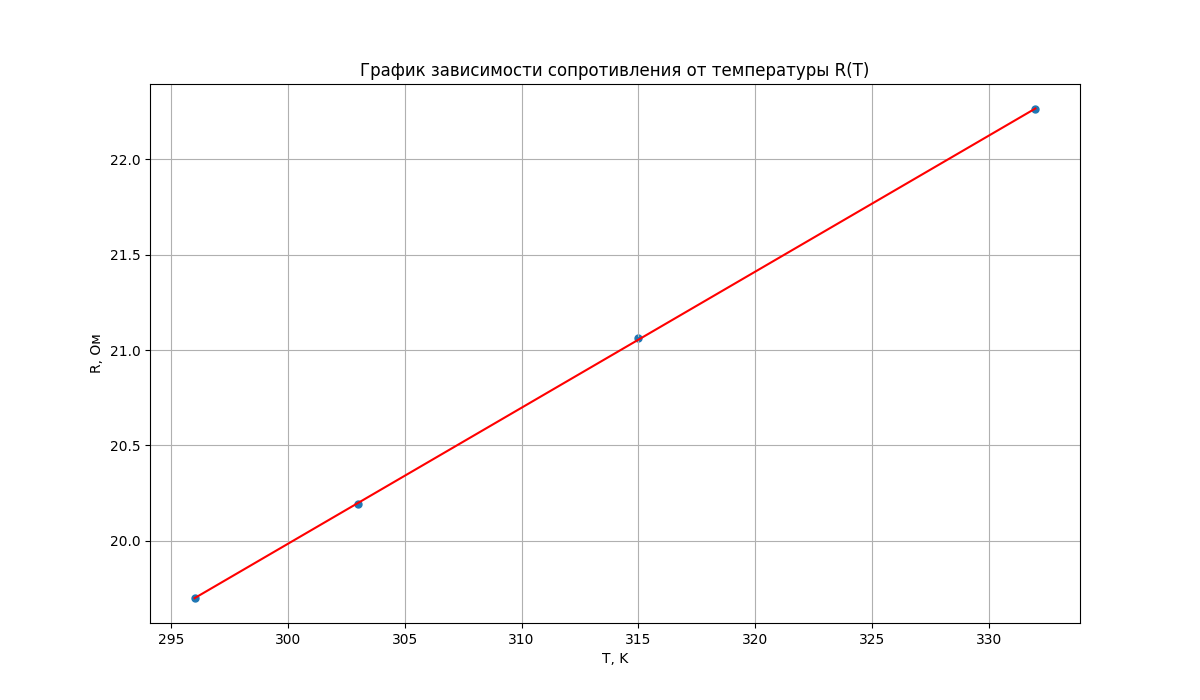
\includegraphics[scale=0.6]{R(T).png}}
                \label{RT_graph}
            \end{figure}

        \subsection{График зависимости теплопроводности воздуха от температуры}

            \ \ \ \ \ \  Используя данные из предыдущих пунктов найдём зависимость выделяющейся на нити мощности $Q$ от её перегрева $\Delta T$ относительно стенок, а также найдём коэффициенты теплопроводности воздуха.

            \[ \frac{dQ}{d(\Delta T)} = \frac{dR_0}{dT} / \frac{dR}{dQ} \ \ \ \ \ \ \ \ \ \ \ \ \ \ \ \ \   k = \frac{dQ}{d(\Delta T)} / \frac{2 \pi L}{ln \frac{r_0}{r_1}} = \frac{dR_0}{dT} \frac{ln \frac{r_0}{r_1}}{2 \pi L} / \frac{dR}{dQ}\]

            \[
            \sigma_k = \sqrt{\left( \frac{\partial k}{\partial \left( \frac{dR_0}{dT} \right)} \sigma_{\frac{dR_0}{dT}} \right)^2 + \left( \frac{\partial k}{\partial \left( \frac{dR}{dQ} \right)} \sigma_{\frac{dR}{dQ}} \right)^2 + \left( \frac{\partial k}{\partial L} \sigma_L \right)^2 + \left( \frac{\partial k}{\partial r_0} \sigma_{r_0} \right)^2 + \left( \frac{\partial k}{\partial r_1} \sigma_{r_1} \right)^2}
        \]

            \begin{table}[!ht]
                \centering
                \begin{tabular}{|c|c|}
                    \hline

                    $t, ^oC$ & $k, 10^{-3}\frac{\text{Вт}}{\text{м} \cdot \text{К}}$\\ \hline
                    $23$ & $(25,57 \pm  0,33)$\\ \hline
                    $30$ & $(26,32 \pm  0,29)$\\ \hline
                    $42$ & $(27,31 \pm  0,39)$\\ \hline
                    $59$ & $(28,56 \pm  0,38)$\\ \hline

                \end{tabular}
                \caption{Коэффициенты теплопроводности воздуха для каждой температуры термостата}
                \label{k_table}
            \end{table}

            Из графика видно, что экспер. значения теплопроводности близки к табличным. \\

            Теперь построим график $ln(k)(ln(T))$.Предполагая, что $k$ степенным образом зависит от абсолютной температуры $T$: $T \sim k^{\beta}$ , построим график в двойном логарифмическом масштабе $ln(k)(ln(T))$  и определите из него показатель степени $\beta$.

            %\newpage

            Построим график зависимости теплопроводности воздуха от температуры и сравним с теоретическим значением. В теории $ \beta = 0.5$, так как коэффициент теплопроводности газа пропорционален корню из температуры. $ \beta_{\text{экс}} = 0.57  $

            \begin{figure}[!ht]
                \center{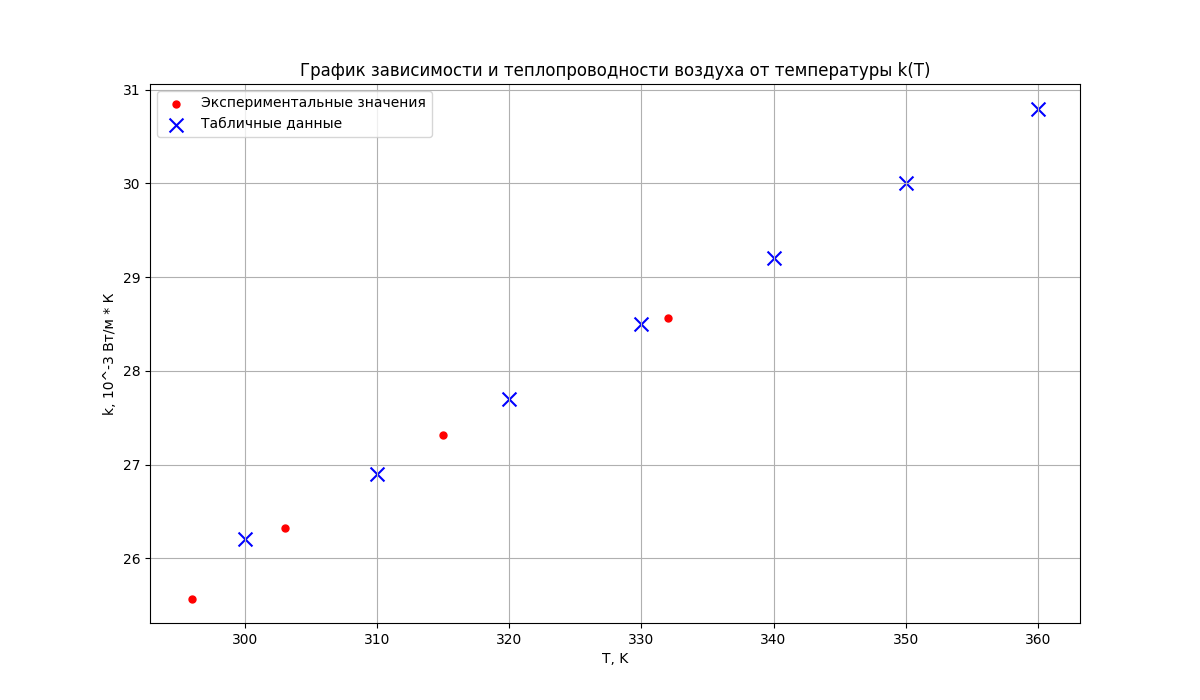
\includegraphics[scale=0.6]{k(T).png}}

                \label{k_graph}
            \end{figure}
          
            \begin{figure}[!ht]
                \center{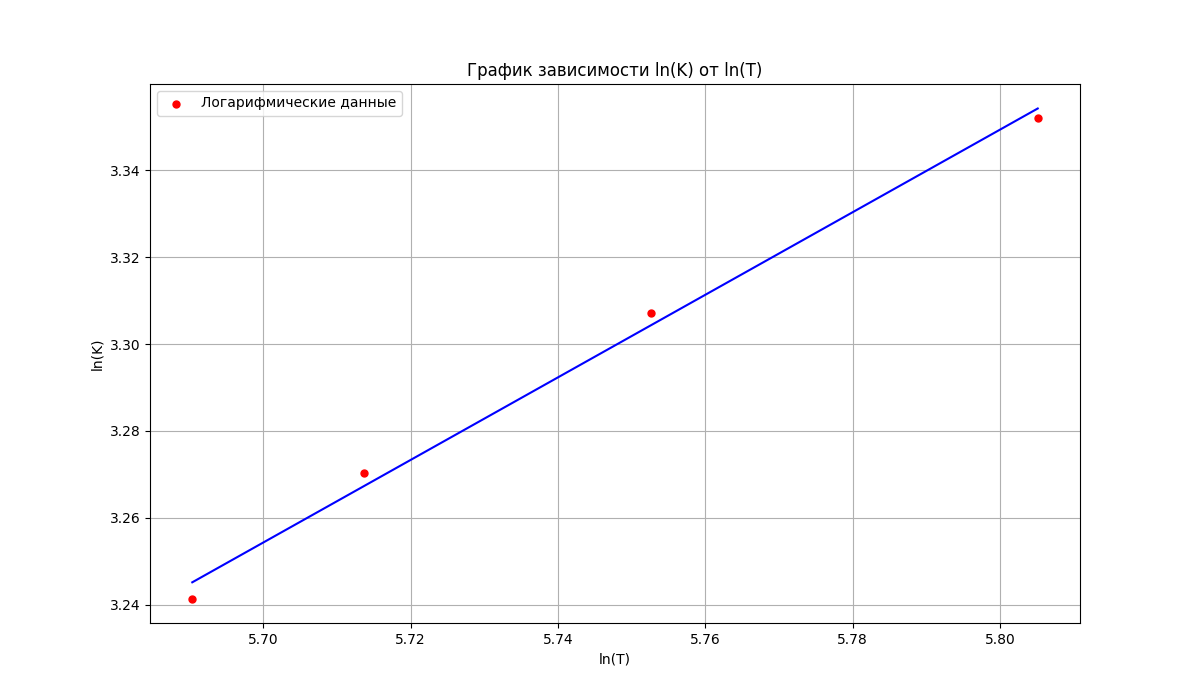
\includegraphics[scale=0.6]{ln_K_ln_T_graph.png}}
                \label{lnk_graph}
            \end{figure}

           


            \section{Выводы}

             В данной работе были измерены зависимости сопротивления платиновой нити от подаваемой на нее мощности при различных температурах. Построены графики зависимости $R(Q)$, получены угловые коэффициенты $\frac{dR}{dQ}$, а также определены сопротивления нити при данных температурах (при $Q \rightarrow 0$).
               Используя полученные значения сопротивления, построен график зависимости сопротивления нити от температуры $R(T)$, а также вычислен температурный коэффициент сопротивления платиновой нити. Экспериментальное значение $\alpha_{\text{эксп}} = 3,948 \pm 0,013 \cdot 10^{-3} \, \text{К}^{-1}$ с относительной погрешностью $\varepsilon_{\alpha} = 0,41\%$ совпадает с теоретическим значением $\alpha_{\text{теор}} = 3,9 \cdot 10^{-3} \, \text{К}^{-1}$.     Были вычислены коэффициенты теплопроводности воздуха при атмосферном давлении и разных температурах. Из графика k(t) можно увидеть, что экспериментальные значения достаточно сильно совпадают с теоретическими.               На графике зависимости $\ln(k)$ от $\ln(T)$ был определен показатель $\beta$. Экспериментальное значение $\beta_{\text{эксп}} = 0,57$ не сильно отличается от теоретического значения $\beta_{\text{теор}} = 0,5$.


\end{document}